\subsection{Compression}

\Fig~\ref{fig:acc_co_wu} illustrates the evaluation results on the dataset altered with compression. It is evident that neither of the networks exhibits robustness to this alteration. In fact, both networks experience an immediate drop in accuracy as the compression level increases, reaching values close to zero. This decline in accuracy is a consequence of the alteration, which significantly alters the image data.
\begin{figure}[H]
	\centering
	\begin{subfigure}{.5\textwidth}
		\centering
		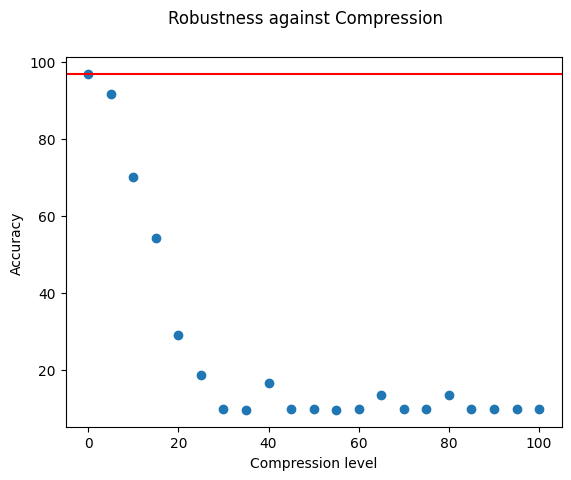
\includegraphics[width=0.9\linewidth]{ImageFiles/EvalBNN/CO/WU/acc}
		\caption{BNN}
		\label{fig:co_acc_wu_bnn}
	\end{subfigure}%
	\begin{subfigure}{.5\textwidth}
		\centering
us		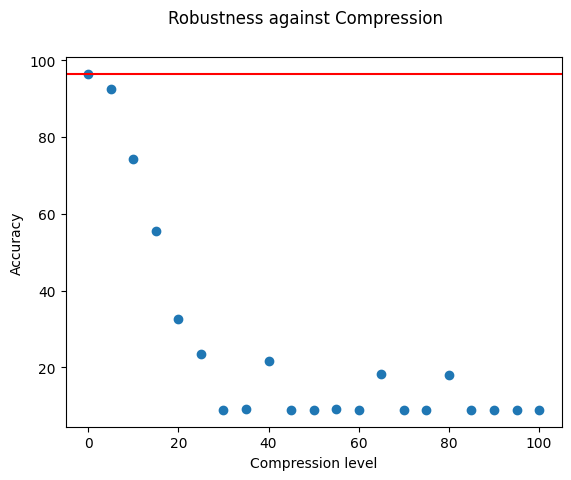
\includegraphics[width=0.9\linewidth]{ImageFiles/EvalANN/compr_ann}
		\caption{Standard NN}
		\label{fig:compr_ann}
	\end{subfigure}
	\caption{Accuracy trend for compression}
	\label{fig:acc_co_wu}
\end{figure}

The robustness metrics computed with this alteration are $0.6208$ for the BNN and $0.6262$ for the standard NN.

In this scenario, both the uncertainties, as shown in \Fig~\ref{fig:co_uncertainty}, exhibit no specific pattern or trend. This suggests a lack of robustness, indicating that the network struggles to identify uncertain situations.
\begin{figure}[H]
	\centering
	\begin{subfigure}{.5\textwidth}
		\centering
		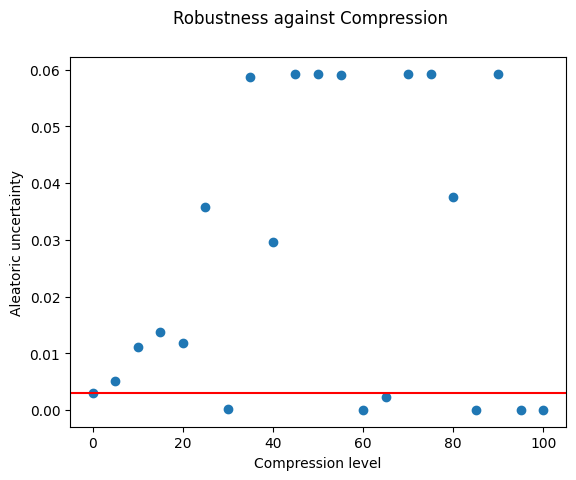
\includegraphics[width=0.9\linewidth]{ImageFiles/EvalBNN/CO/aleatoric}
		\caption{Aleatoric uncertainty}
		\label{fig:co_aleatoric}
	\end{subfigure}%
	\begin{subfigure}{.5\textwidth}
		\centering
		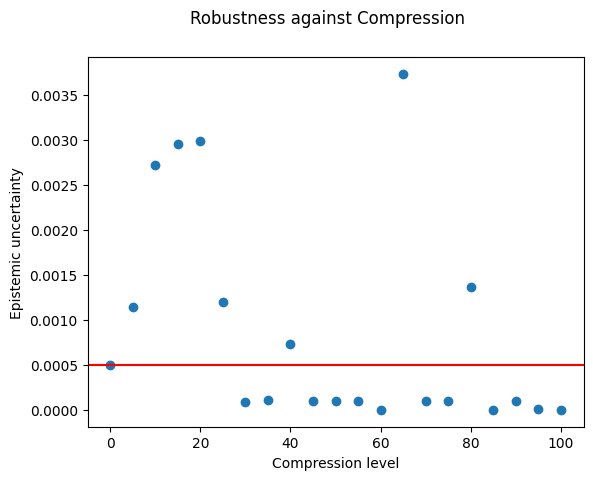
\includegraphics[width=0.9\linewidth]{ImageFiles/EvalBNN/CO/epistemic}
		\caption{Epistemic uncertainty}
		\label{fig:co_epistemic}
	\end{subfigure}
	\caption{Uncertainty trend for compression}
	\label{fig:co_uncertainty}
\end{figure}

\vspace{0.3cm}
\textbf{Classification using aleatoric uncertainty}
\vspace{0.1cm}

The utilization of aleatoric uncertainty does not lead to an improved performance, as evidenced in \Fig~\ref{fig:co_au}. However, it is worth noting that the accuracy, as shown in \Fig~\ref{fig:co_au_acc}, occasionally reaches $100\%$ for certain alteration levels. This is due to the fact that the unknown ratio values reach $100\%$, as seen in \Fig~\ref{fig:co_au_unkn}. In such cases, the uncertainty is conventionally set to the maximum value, as there are no actual predictions; only unknown values are present. This highlights the network inability to effectively handle this alteration. This behavior is further illustrated by the effectiveness metric in \Fig~\ref{fig:co_au_eff}.
\begin{figure}[H]
	\centering
	\begin{subfigure}{.33\textwidth}
		\centering
		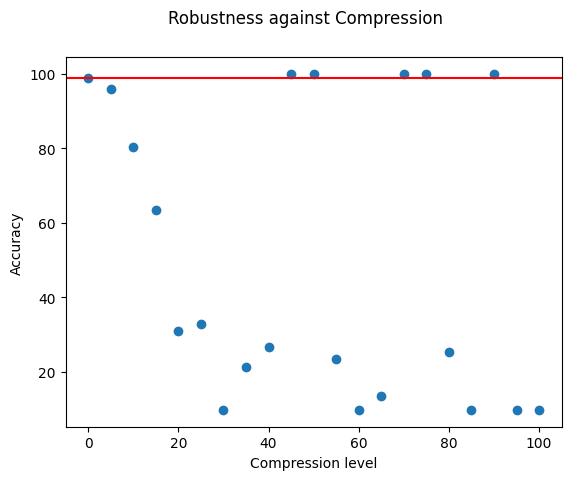
\includegraphics[width=0.9\linewidth]{ImageFiles/EvalBNN/CO/AU/acc}
		\caption{Accuracy using aleatoric \\ uncertainty}
		\label{fig:co_au_acc}
	\end{subfigure}%
	\begin{subfigure}{.33\textwidth}
		\centering
		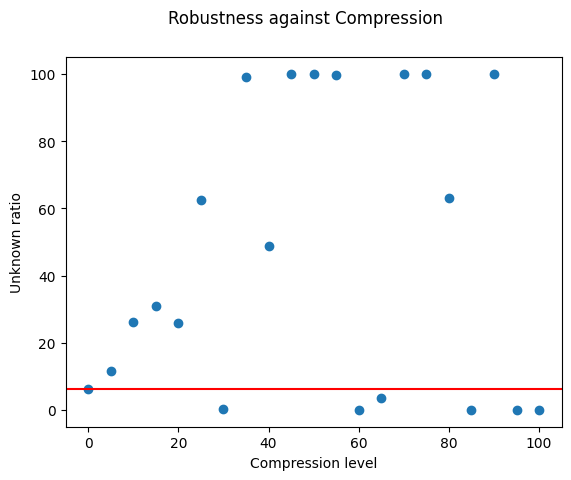
\includegraphics[width=0.9\linewidth]{ImageFiles/EvalBNN/CO/AU/unkn}
		\caption{Unknown ratio using aleatoric uncertainty}
		\label{fig:co_au_unkn}
	\end{subfigure}%
	\begin{subfigure}{.33\textwidth}
		\centering
		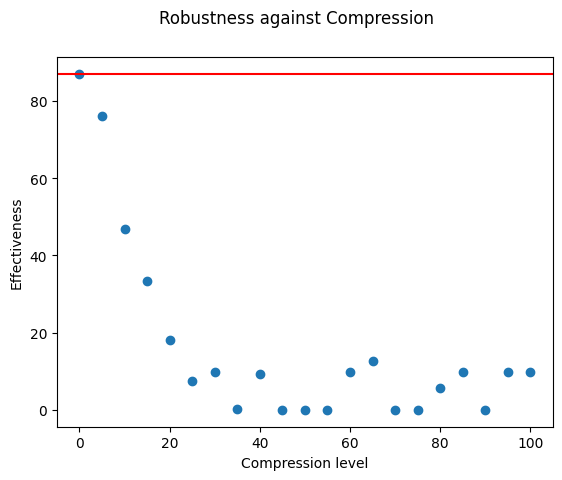
\includegraphics[width=0.9\linewidth]{ImageFiles/EvalBNN/CO/AU/eff}
		\caption{Effectiveness using aleatoric uncertainty}
		\label{fig:co_au_eff}
	\end{subfigure}
	\caption{Robustness graph for compression when aleatoric uncertainty is employed in the classification}
	\label{fig:co_au}
\end{figure}

\Tab~\ref{table:rob_co_au} presents the quantitative robustness measurements.
\begin{table}[h]
	\centering
	\begin{tabular}{|| l | l ||} 
		\hline
		\textbf{Parameter} & \textbf{Value} \\
		\hline
		\hline
		$rob_{Compression}$ & $0.7533$ \\
		$robInd_{Compression}$ & $0.7655$ \\
		$robAug_{Compression}$ & $0.5854$ \\	
		\hline
	\end{tabular}	
	\caption{Robustness metrics for compression when the aleatoric uncertainty is employed}
	\label{table:rob_co_au}
\end{table}

\vspace{0.3cm}
\textbf{Classification using epistemic uncertainty}
\vspace{0.1cm}

\Fig~\ref{fig:co_eu} illustrates the evaluation results using epistemic uncertainty. The accuracy trend, as shown in \Fig~\ref{fig:co_eu_acc}, does not exhibit any significant difference compared to the scenario without the use of uncertainty. This suggests that epistemic uncertainty is unable to identify uncertain situations effectively.

\begin{figure}[H]
	\centering
	\begin{subfigure}{.33\textwidth}
		\centering
		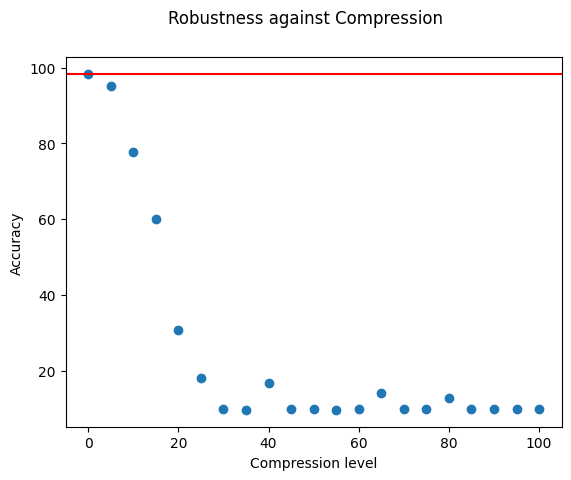
\includegraphics[width=0.9\linewidth]{ImageFiles/EvalBNN/CO/EU/acc}
		\caption{Accuracy using epistemic \\ uncertainty}
		\label{fig:co_eu_acc}
	\end{subfigure}%
	\begin{subfigure}{.33\textwidth}
		\centering
		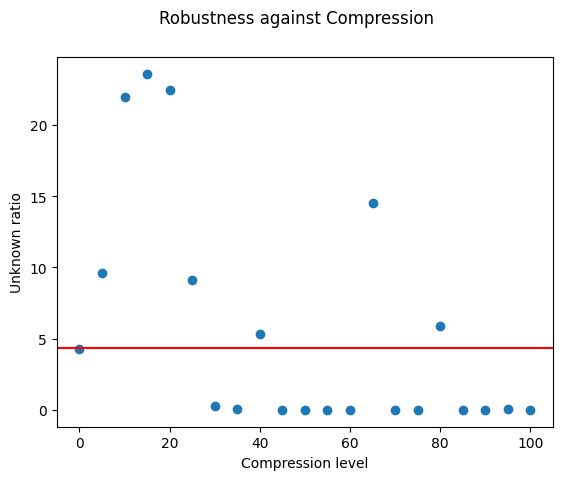
\includegraphics[width=0.9\linewidth]{ImageFiles/EvalBNN/CO/EU/unkn}
		\caption{Unknown ratio using \\ epistemic uncertainty}
		\label{fig:co_eu_unkn}
	\end{subfigure}%
	\begin{subfigure}{.33\textwidth}
		\centering
		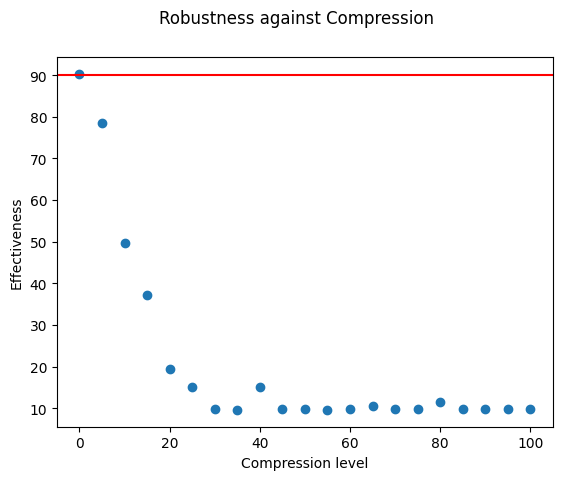
\includegraphics[width=0.9\linewidth]{ImageFiles/EvalBNN/CO/EU/eff}
		\caption{Effectiveness using \\ epistemic uncertainty}
		\label{fig:co_eu_eff}
	\end{subfigure}
	\caption{Robustness graph for compression when epistemic uncertainty is employed in the classification}
	\label{fig:co_eu}
\end{figure}

\Tab~\ref{table:rob_co_eu} displays the robustness metrics.

\begin{table}[H]
	\centering
	\begin{tabular}{|| l | l ||} 
		\hline
		\textbf{Parameter} & \textbf{Value} \\
		\hline
		\hline
		$rob_{Compression}$ & $0.6238$ \\
		$robInd_{Compression}$ & $0.9797$ \\
		$robAug_{Compression}$ & $0.6093$ \\	
		\hline
	\end{tabular}	
	\caption{Robustness metrics for compression alteration when the epistemic uncertainty is employed}
	\label{table:rob_co_eu}
\end{table}

\vspace{0.3cm}
\textbf{Classification using standard deviation}
\vspace{0.1cm}

The results obtained when using standard deviation, as illustrated in \Fig~\ref{fig:co_vu}, exhibit the same behavior as when using aleatoric uncertainty.

\begin{figure}[H]
	\centering
	\begin{subfigure}{.33\textwidth}
		\centering
		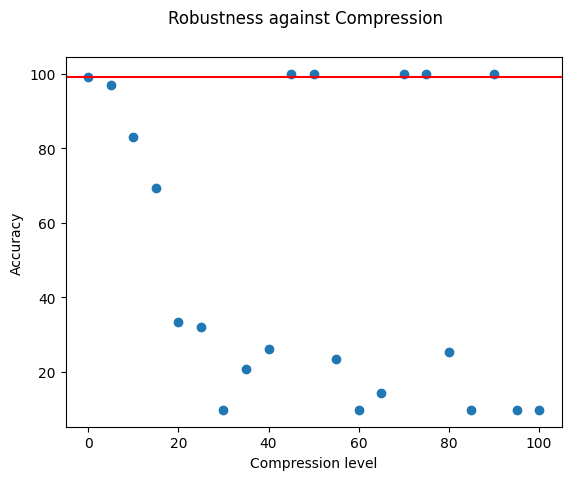
\includegraphics[width=0.9\linewidth]{ImageFiles/EvalBNN/CO/VU/acc}
		\caption{Accuracy using standard \\ deviation}
		\label{fig:co_vu_acc}
	\end{subfigure}%
	\begin{subfigure}{.33\textwidth}
		\centering
		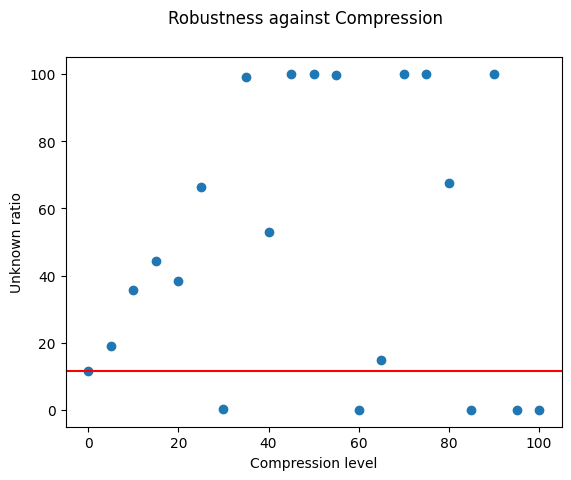
\includegraphics[width=0.9\linewidth]{ImageFiles/EvalBNN/CO/VU/unkn}
		\caption{Unknown ratio using \\ standard deviation}
		\label{fig:co_vu_unkn}
	\end{subfigure}%
	\begin{subfigure}{.33\textwidth}
		\centering
		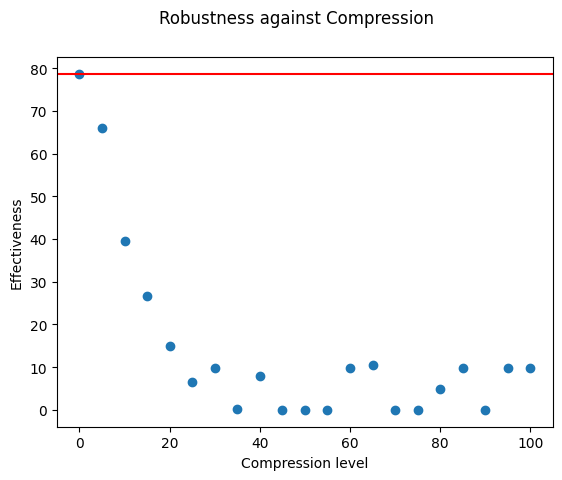
\includegraphics[width=0.9\linewidth]{ImageFiles/EvalBNN/CO/VU/eff}
		\caption{Effectiveness using standard deviation}
		\label{fig:co_vu_eff}
	\end{subfigure}
	\caption{Robustness graph for compression when standard deviation is employed in the classification}
	\label{fig:co_vu}
\end{figure}

\Tab~\ref{table:rob_co_vu} gives the quantitative robustness measurements.

\begin{table}[H]
	\centering
	\begin{tabular}{|| l | l ||} 
		\hline
		\textbf{Parameter} & \textbf{Value} \\
		\hline
		\hline
		$rob_{Compression}$ & $0.7586$ \\
		$robInd_{Compression}$ & $0.7558$ \\
		$robAug_{Compression}$ & $0.5674$ \\	
		\hline
	\end{tabular}	
	\caption{Robustness metrics for compression when the standard deviation is employed}
	\label{table:rob_co_vu}
\end{table}

\vspace{0.3cm}
\textbf{Comparison}
\vspace{0.1cm}

Table~\ref{table:rob_co} presents a comparison of the computed metrics. It is evident that the network lacks robustness for any uncertainty type. In this scenario, a possible solution could be to change the network architecture or employ techniques for improving robustness, such as \textit{data augmentation}. Additionally, revising the alteration range and conducting another domain analysis may also be beneficial as the robustness is defined with respect to an alteration range.

\begin{table}[H]
	\centering
	\begin{tabular}{|| l | l | l | l ||} 
		\hline
		\textbf{Parameter} & \textbf{Aleatoric} & \textbf{Epistemic} & \textbf{Standard deviation} \\
		\hline
		\hline
		$rob_{Compression}$ & $0.7533$ & $0.6238$ & $0.7586$ \\
		$robInd_{Compression}$ & $0.7655$ & $0.9797$ & $0.7558$ \\
		$robAug_{Compression}$ & $0.5854$ & $0.6093$ & $0.5674$ \\	
		\hline
	\end{tabular}	
	\caption{Summary of the robustness metrics for compression}
	\label{table:rob_co}
\end{table}